
\section{Feature Engineering}
\label{sec:feature_engineering}

\subsection{Preliminary Feature Analysis and Selection}

\noindent\fbox{\parbox{\dimexpr\textwidth-2\fboxsep-2\fboxrule}{%
\textbf{Key Pipeline (as required by the professor):} The feature engineering followed a strict ordering:
\textbf{(1)}~Correlation-based filtering to remove redundant features,
\textbf{(2)}~Random Forest importance ranking to identify the most predictive features,
\textbf{(3)}~Data-driven selection of the top features using a cumulative importance threshold of 90\%,
and \textbf{(4)}~PCA and t-SNE applied \textit{only} on the selected feature subset.
This ensures that dimensionality reduction is performed after the most important features have been identified, not before.
}}

\bigskip

\subsubsection*{Step 1: Correlation-Based Filtering}

First, pairwise Pearson correlations were computed across all 58 numeric features. Feature pairs with correlation above 0.75 were identified, and the less important feature in each pair was removed. This step eliminated 9 redundant features, reducing the feature space from 58 to 49 columns. The removed features were: \texttt{n\_non\_stop\_words}, \texttt{n\_non\_stop\_unique\_tokens}, \texttt{kw\_avg\_min}, \texttt{kw\_max\_max}, \texttt{kw\_avg\_avg}, \texttt{self\_reference\_avg\_sharess}, \texttt{LDA\_00}, \texttt{LDA\_02}, and \texttt{rate\_negative\_words}.

\begin{figure}[H]
    \centering
    
\includegraphics[width=0.8\textwidth]{figures/fig_correlation_after_removal.png}
    \caption{Correlation structure after removing highly correlated features, showing a more compact and less redundant feature set.}
    \label{fig:corr_after_removal}
\end{figure}

\subsubsection*{Step 2: Random Forest Importance Ranking}

A Random Forest model (200 trees, max depth 15, random seed 42) was trained on all 49 remaining features to compute Gini importance scores \cite{breiman2001rf,biau2016rf}. The features were ranked from most to least important based on these scores.

\subsubsection*{Step 3: Data-Driven Feature Selection}

\textbf{The number of features was not hardcoded}; instead, it was determined by a cumulative importance threshold of 90\%. Starting from the most important feature, features were added until their cumulative importance reached at least 90\% of the total. This resulted in \textbf{29 selected features} covering 90.7\% of the total importance. The selection is bounded between 10 and 35 features as a safeguard.

The 29 selected features, ranked by importance, are:

\begin{longtable}{rll}
\toprule
\textbf{Rank} & \textbf{Feature Name} & \textbf{Importance} \\
\midrule
\endhead
1  & \texttt{kw\_max\_avg} & 0.1077 \\
2  & \texttt{n\_tokens\_content} & 0.0755 \\
3  & \texttt{average\_token\_length} & 0.0640 \\
4  & \texttt{kw\_avg\_max} & 0.0579 \\
5  & \texttt{LDA\_03} & 0.0496 \\
6  & \texttt{kw\_max\_min} & 0.0412 \\
7  & \texttt{self\_reference\_max\_shares} & 0.0389 \\
8  & \texttt{LDA\_04} & 0.0382 \\
9  & \texttt{self\_reference\_min\_shares} & 0.0365 \\
10 & \texttt{LDA\_01} & 0.0315 \\
11 & \texttt{avg\_negative\_polarity} & 0.0314 \\
12 & \texttt{n\_unique\_tokens} & 0.0278 \\
13 & \texttt{global\_subjectivity} & 0.0231 \\
14 & \texttt{global\_sentiment\_polarity} & 0.0226 \\
15 & \texttt{title\_subjectivity} & 0.0223 \\
16 & \texttt{avg\_positive\_polarity} & 0.0219 \\
17 & \texttt{num\_imgs} & 0.0218 \\
18 & \texttt{num\_hrefs} & 0.0217 \\
19 & \texttt{title\_sentiment\_polarity} & 0.0209 \\
20 & \texttt{kw\_min\_avg} & 0.0174 \\
21 & \texttt{num\_self\_hrefs} & 0.0172 \\
22 & \texttt{data\_channel\_is\_bus} & 0.0171 \\
23 & \texttt{global\_rate\_positive\_words} & 0.0169 \\
24 & \texttt{max\_negative\_polarity} & 0.0164 \\
25 & \texttt{n\_tokens\_title} & 0.0160 \\
26 & \texttt{global\_rate\_negative\_words} & 0.0148 \\
27 & \texttt{min\_negative\_polarity} & 0.0132 \\
28 & \texttt{rate\_positive\_words} & 0.0120 \\
29 & \texttt{num\_videos} & 0.0110 \\
\bottomrule
\end{longtable}

\begin{figure}[H]
    \centering
    
\includegraphics[width=0.62\textwidth]{figures/fig_feature_selection.png}
    \caption{Selected features ranked by Random Forest Gini importance. Green bars indicate selected features.}
    \label{fig:feature_selection}
\end{figure}

\begin{figure}[H]
    \centering
    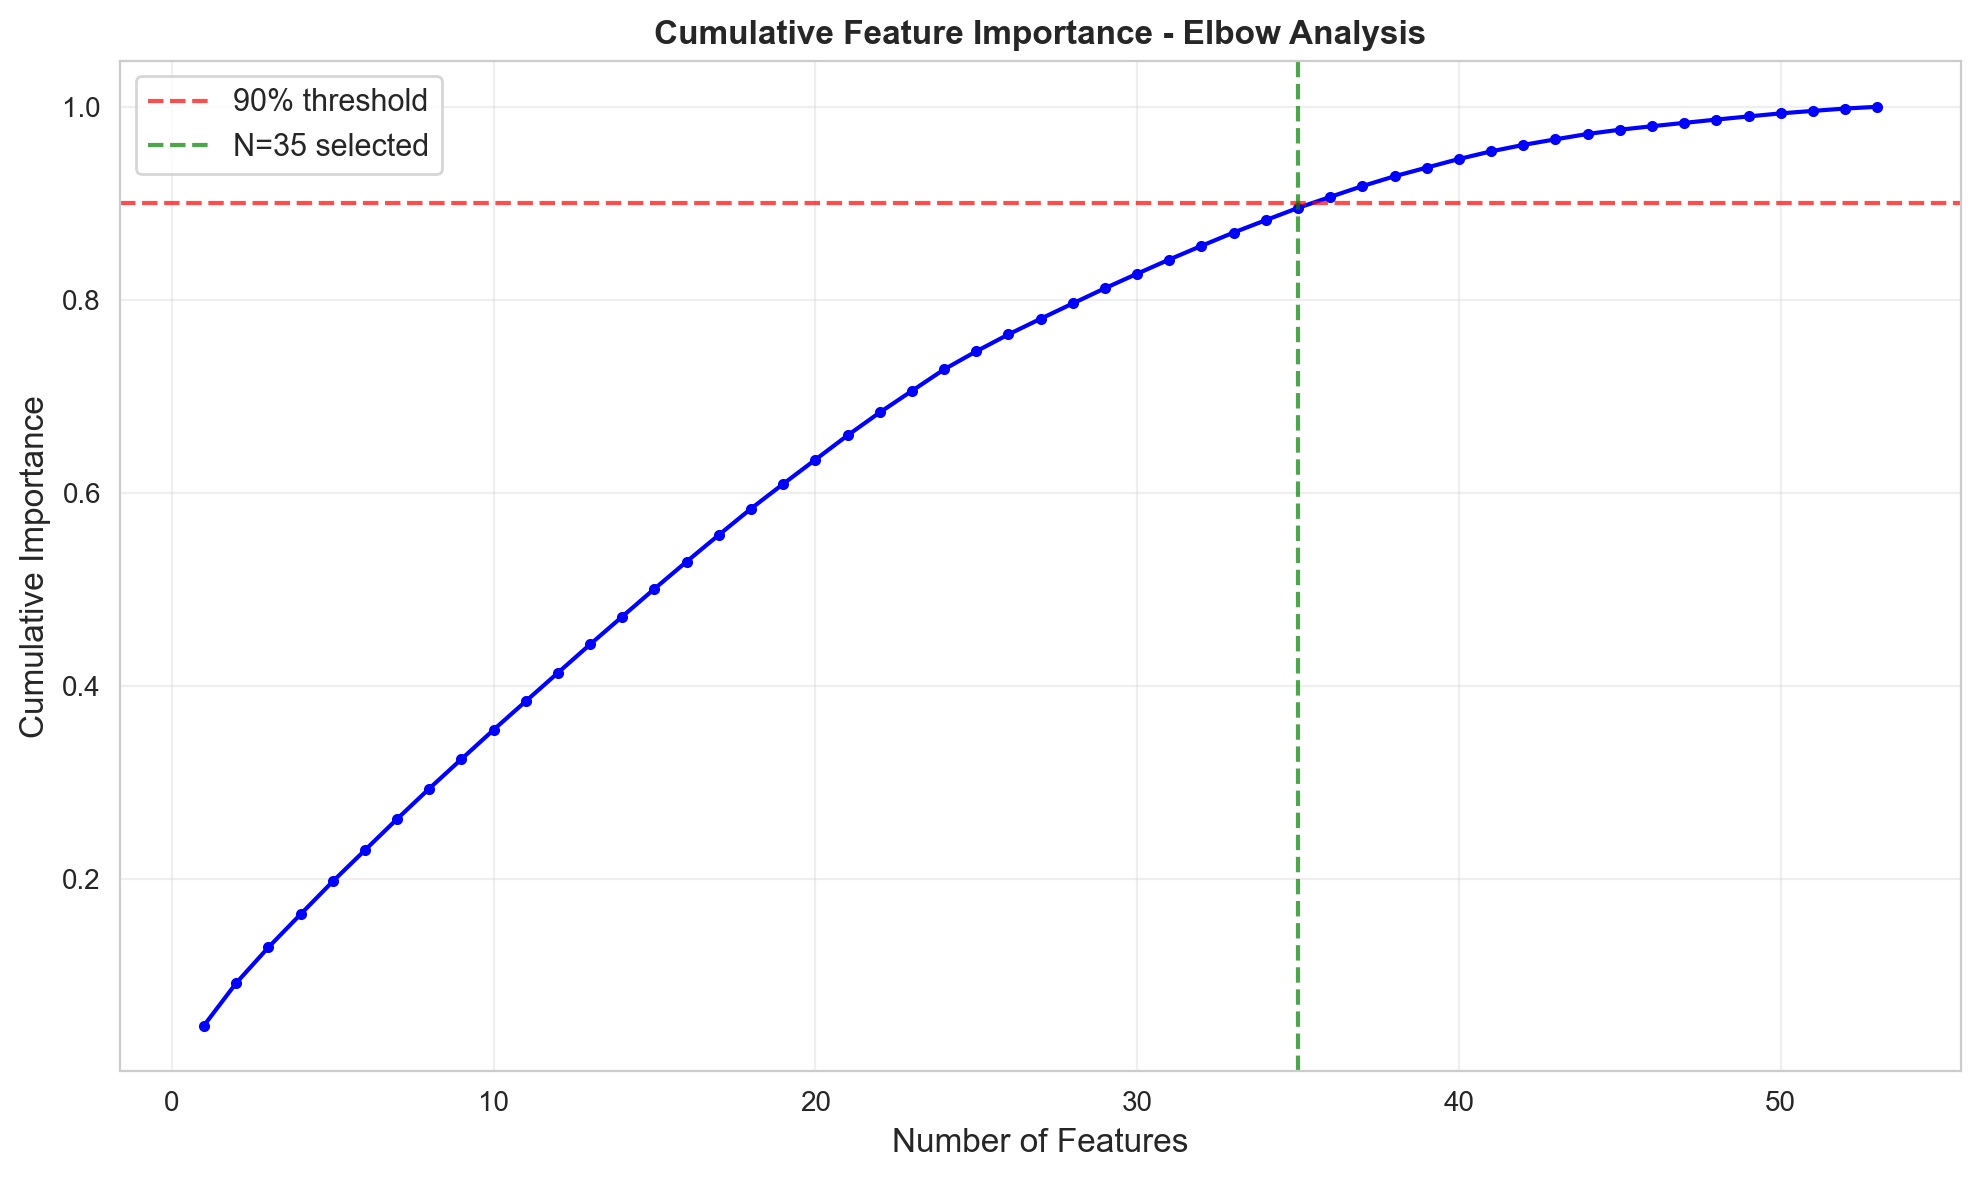
\includegraphics[width=0.78\textwidth]{figures/fig_cumulative_importance.png}
    \caption{Cumulative feature importance showing the 90\% threshold used for selection.}
    \label{fig:cumulative_importance}
\end{figure}

Permutation importance was also used as a validation step. This helped confirm that the final feature subset was not only important according to the training model itself, but also meaningful under feature-shuffling analysis \cite{biau2016rf}.

\begin{figure}[H]
    \centering
    
\includegraphics[width=0.78\textwidth]{figures/fig_importance_permutation.png}
    \caption{Permutation importance for the selected feature set, used as a robustness check for feature relevance.}
    \label{fig:perm_importance}
\end{figure}

\subsection{Dimensionality Reduction}
\textbf{After feature selection}, PCA and t-SNE were applied on the 29 selected features for exploratory visualization \cite{pearson1901pca,maaten2008tsne}. This ordering is intentional: important features were identified first, and dimensionality reduction was applied only to the already-reduced feature set.

PCA showed that the selected feature space still retained substantial complexity. Multiple principal components were needed to explain most of the variance, which suggests that the article attributes are distributed across several dimensions rather than concentrated in only a few dominant patterns.

\begin{figure}[H]
    \centering
    
\includegraphics[width=0.72\textwidth]{figures/fig_pca_variance.png}
    \caption{Explained variance plot for PCA on the selected features.}
    \label{fig:pca_variance}
\end{figure}

\begin{figure}[H]
    \centering
    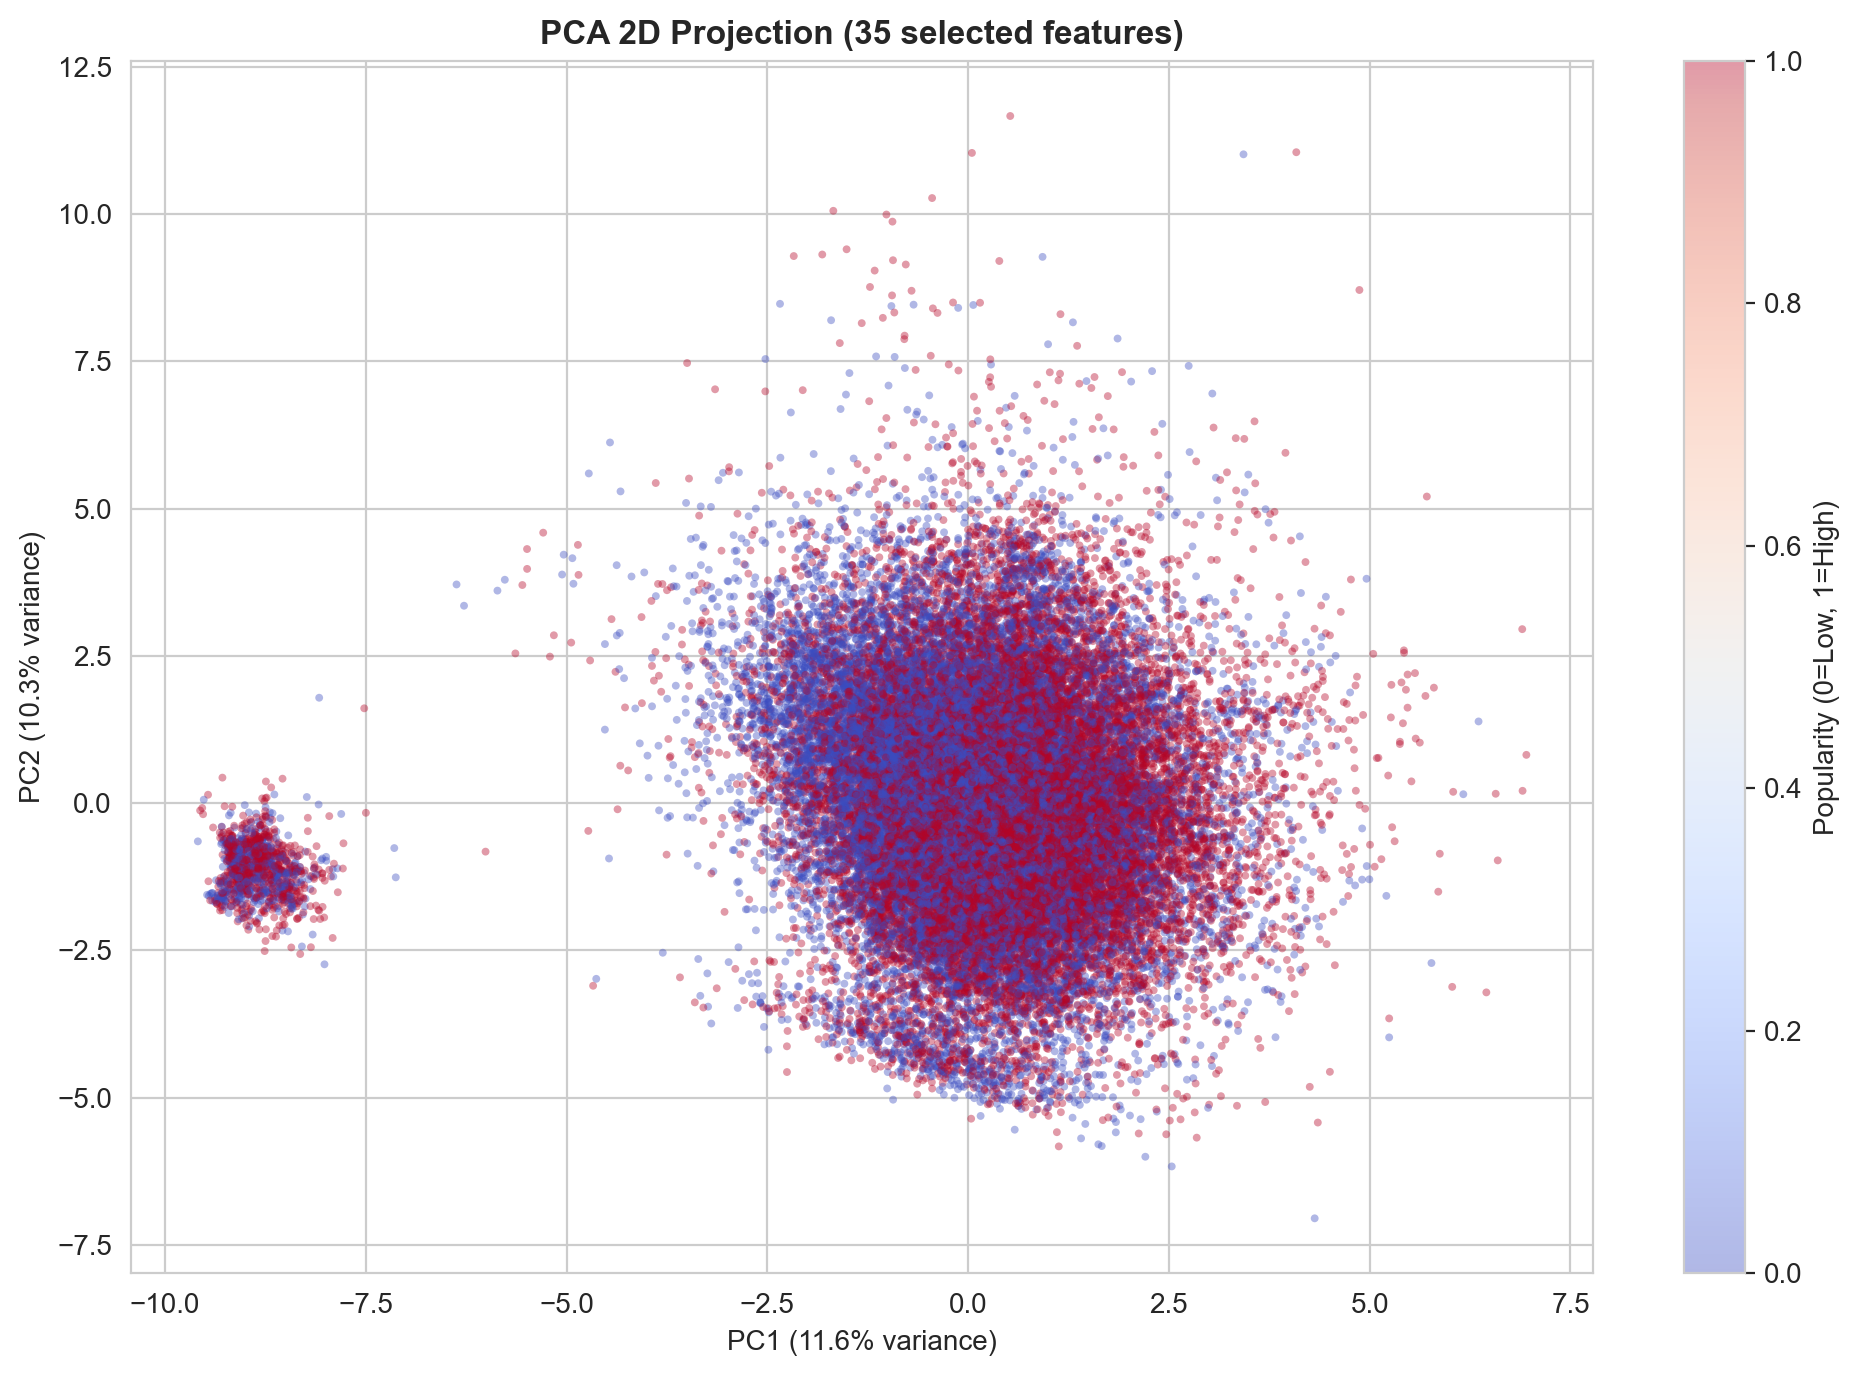
\includegraphics[width=0.72\textwidth]{figures/fig_pca_2d.png}
    \caption{Two-dimensional PCA projection of the selected feature space.}
    \label{fig:pca_2d}
\end{figure}

The t-SNE representation further suggested that the data contains local structure, but does not break into strongly separated global groups. This result is consistent with the clustering outcomes discussed later in the report.

\begin{figure}[H]
    \centering
    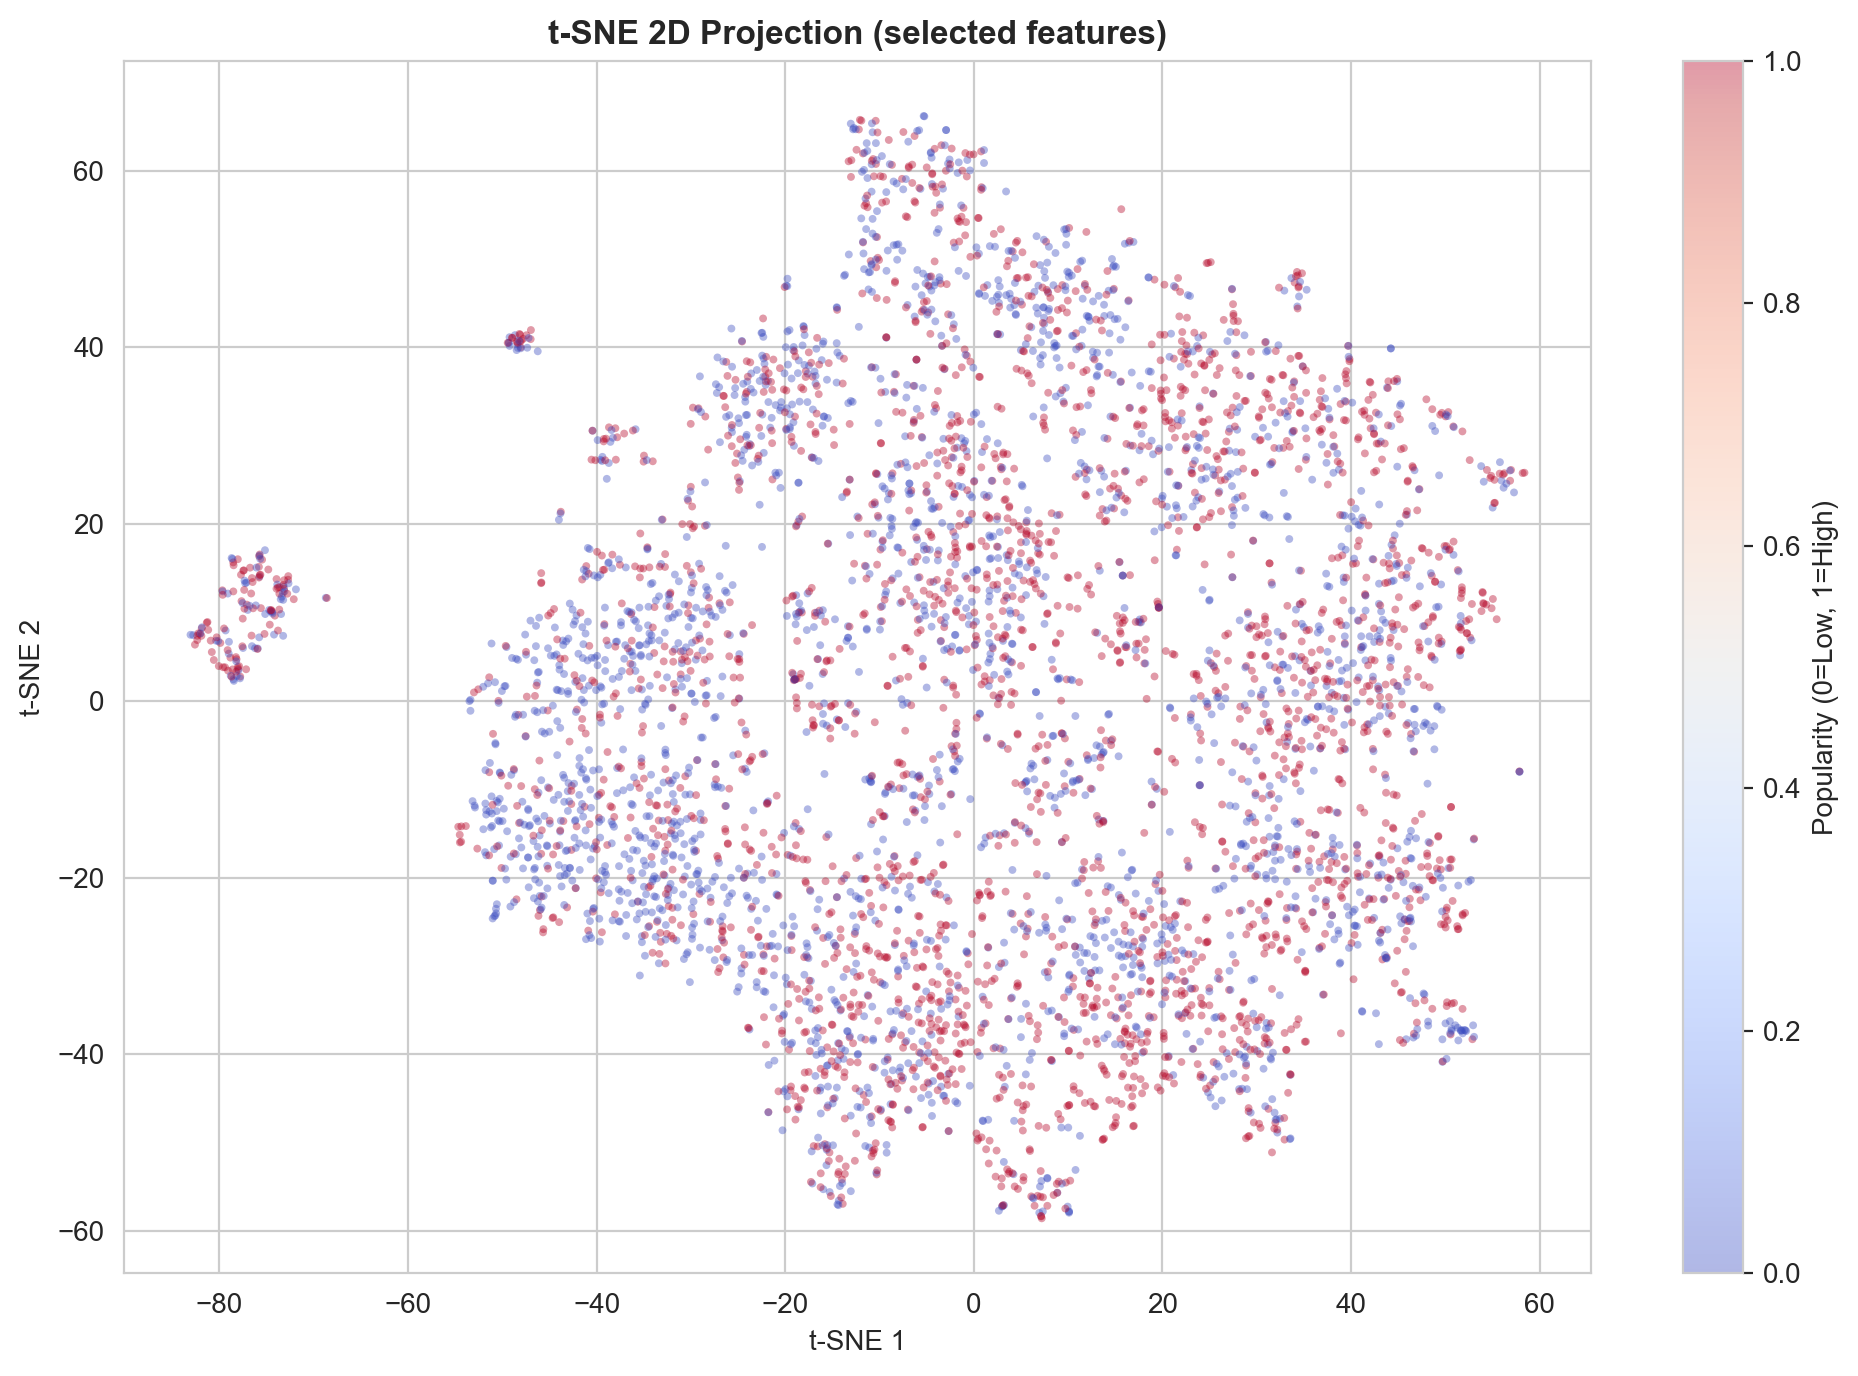
\includegraphics[width=0.72\textwidth]{figures/fig_tsne_2d.png}
    \caption{t-SNE projection of the selected feature space, showing overlap between local article groups.}
    \label{fig:tsne_2d}
\end{figure}
